

\chapter{Litterature review}
\section{Context: mountain grasslands and climate change}

\begin{figure*}

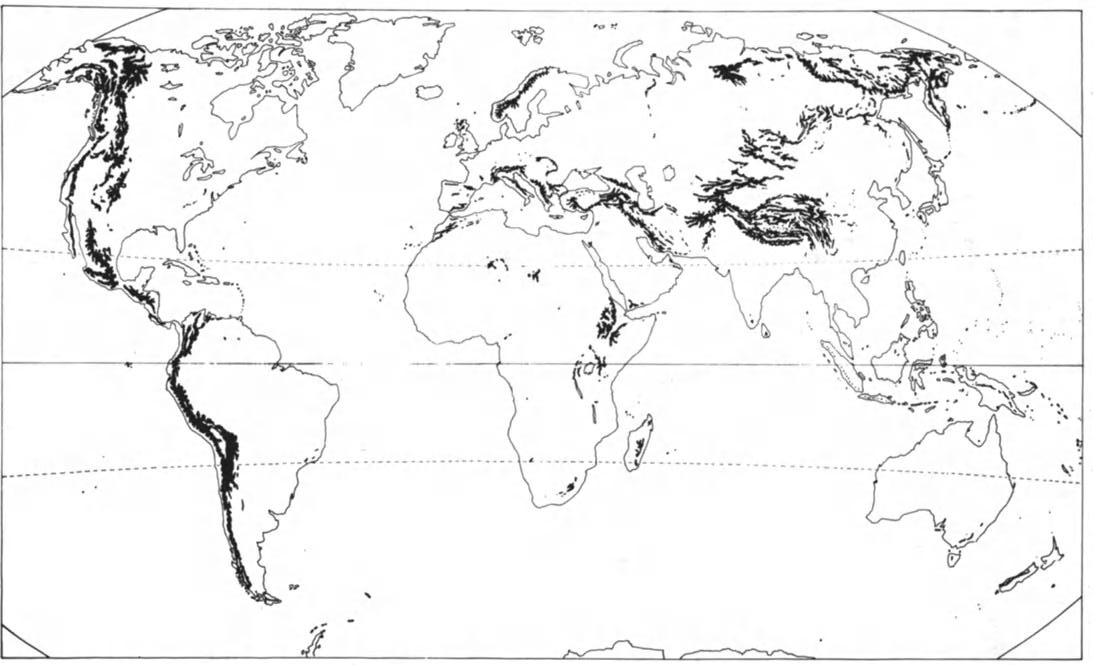
\includegraphics{./1_Introduction/graphics/alpine_distribution.jpeg}
\caption{Distribution of alpine habitats}
\end{figure*}

\section{Diversity and coexistence mechanisms}
Why interested in diversity? precious, main objective in conservation, plus services. Why coexistence mechanisms? Mechanism at plant level that allow diversity, understanding these will help us predict changes in diversity.

\subsection{Effects of diversity}
Conservation\\
productivity\\
resistance ?\\
Ecosystem services and complementarity\\

\subsection{Mechanisms for coexistence and strategies}
main theories: niche, neutral, individual based. -> scale and dimension dependant.\\
chesson \cite{chesson_mechanisms_2000}\\
Spatial and temporal variability\\
trade-off, strategy space, and variability.\\
in the end it's rarely direct interaction but capacity to respond to stress and interect interaction through resource pools.

\paragraph{Strategy space and trade-off}

\paragraph{about trade-off}
chemical physical trade-off vs ecological trade-off.

\section{global change and community dynamics: theory and empirical results}

\subsection{Community dynamics: from individuals to group dynamics}
\textbf{Need to  highligth how community dynamics emerge from individual response and interactions.}

\subsection{Intraspecific variability}
frame of reference: deep traits vs shallow traits. definition of functional trait.\\
source of intra specific variability: genetic vs ontogeny vs plasticity (epigen) \\
effect on niche and interactions: effect on coexistence\\
-> plasticity a special form of ISV
\subsection{Understanding phenotypic plasticity}
adaptive intraspecific variation\\
cost and limits van kleunen, Dewitt and sultan \\
effect on coexistence and community


\section{Existing  modelling solutions and approaches to question global change effect on vegetation community}

Message: modelling coexistence is a challenge because 1) do not know/understand all mechanisms, 2) challenging to incorporate enough mechanisms, 3) costly computation and data wise. -> need for more generic and complete (multiple mechanisms approaches.\\

DGVMs\\
IBMs

Reaction norms\\
Source sink models\\
Functional-Structural plant models FSPMs ? vos 2009\\
Functional equilibrium. Somehow similar to the source sink in its philosophy, it allows optimisation of phenotype for multiple resources. \\


\subsection{Modelling vegetation - traits and strategies}
traits \& strategies\\
existing models: a gap to fill\\
coexistence processes

%
%
%%_________________________________________________________________________________
%\chapter{Mountain grasslands}
%\fwnewthought{Mountain grasslands have an unique beauty drawn by the diversity of flowers colours, the strong contrast between the luxurious green vegetation and the roughness of the naked rocks, and the feeling that living in such places, at the edge of living conditions, is a fight worth fighting. I could illustrate this beauty with thousands pictures and words, and it would certainly convince you that these ecosystems worth spending time studying them to better understand and protect them. I could also describe their role in the economy of alpine regions, currently subject of great modification, and greater to come. But you would not see these rich systems as I see them: as an intricate network of interaction living creatures, with their own characteristics, strategy and experience, forming a dynamic system... Capturing this beauty is one challenge of this modelling PhD.\\
%I must now give you an overview on the mountain grasslands}
%
%
%%\section{Photograph of mountain grasslands}
%The idea is to go from context, to services to ecology. At the entd of this part, it is obvious that ecosystem services can be derived from traits and that we need tools for prediction of MG dynamics.
%
%\section{Geography, climate and managements: les drivers}
%
%
%\section{Mountain grasslands under climate change}
%
%\section{Mountain grasslands, source of services}
%
%\section{Let's talk about traits} % might not be at the right place here
%response trait and effect traits (?) <- you need to talk about this to better introduce the shift from there to a deep/low level traits to composite traits (SLA if related to a certain resource use strategy, is also a composite trait (Nitrogen, light and water all affect the SLA value). View such traits as mono dimensional is dangerous as it simplify a lot (and I might have fallen within this trap). Having low level traits that define the overall strategy (and not how to achieve it) should help to have a more systemic view (good term here ? view of the system with all its parts) and better understand the rules that drive the development. But they also imply the need for new mechanisms to link such traits and strategies to actual, measurable traits that define the phenotype as we see it (at the level of interaction or services profides). \\
%Opportunity to emphasis the fact (a simple scheme should help here) that apparent traits are usefull (and measurable) to define the current effect on the environment (and so interactions between plants) and on provided services, but they are difficult to use to predict the dynamic of individuals and communities (precisely because they are changing and composit traits that respond to the environment).
%
%
%
%%_________________________________________________________________________________
%\chapter{Modelling ecological systems}
%The message here should be that: we know how to model vegetation systems, but we need finer resolution (from species and com, to traits, to individual responses) and bigger (higher number of species) scale -> generic framework and individual response.\\
%Based on two particular similar models: taubert, and Lohier.
%
%\section{Models as understanding and testing tools}
%
%\begin{quote}
%"Physicien de la biologie"
%\end{quote}
%Justify the modelling approach - what's a model ? simplification of reality\\
%Long subject refer to models in ecosystem sciences. Different classes of model, and different objectives. Mechanistic models: understanding and testing hypothesis.\\
%Model as understanding tools: how does modelling help us understanding the system we are modelling.\\
%The need for mechanistic model and emergent properties of models. Process-based models vs statistical model (what happen outside the data (example of flickering tails of regression models), similar to bayesian approach, the model is constrained by our understanding of processes.) \\
%mechanistic models: risks of lack of mechanisms, complex calibration, lot of parameters. Statistical model have the advantage of parcymony: minimum number of parameters to reproduce a pattern.
%
%\section{Modelling plant communities}
%
%\subsection{Different levels of modelling: from communities to individuals}
%community approaches, CWM to importance of individuals.\\
%
%
%\subsection{Processes}
%\paragraph{Test pragraph title - now what happen if it lays on multiples lines} This is a paragraphe \lipsum[2]
%
%\marginnote{\textbf{some notes}}
%\marginnote{\lipsum[1]}
%\sidenote{a short sidenote}
%
%\subsection{Agent-based models}
%
%Review of existing models (grasslands and forest)\\
%Comparison of two existing models\\
%How to build aroung/from that.\\
%
%
%\section{Modelling coexistence}
%Message: modelling coexistence is a challenge because 1) do not know/understand all mechanisms, 2) challenging to incorporate enough mechanisms, 3) costly computation and data wise. -> need for more generic and complete (multiple mechanisms approaches.
%
%\subsection{What is diversity and why model it?}
%
%On why model coxistence: better understanding of mechanisms, tool to evaluate and predict changes in coexistence.
%
%\begin{figure}
%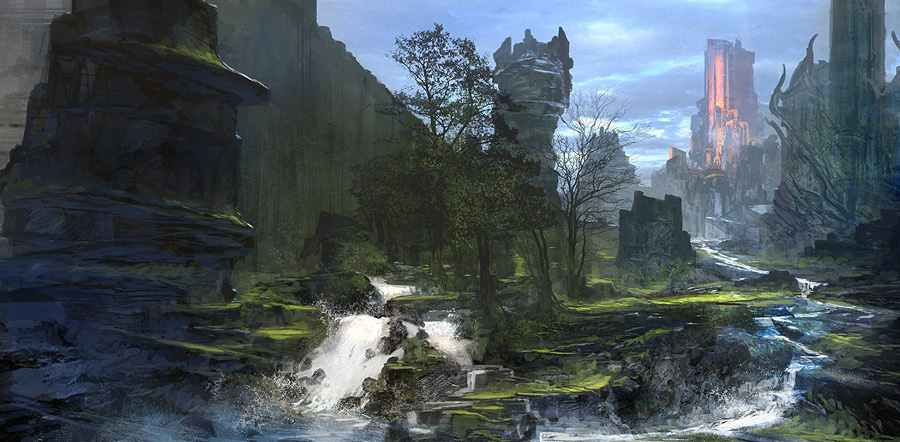
\includegraphics[scale=1]{./1_Introduction/graphics/plankton.jpg}
%\end{figure}
%
%\subsection{The concept of niche}
%
%
%\subsection{Coexistence mechanisms}
%
%\section{Breaking the resolution-specificity trade-off}
%use of generic species\\
%still a trade-off with scale.
%
%%_________________________________________________________________________________
%\chapter{Phenotypic plasticity of organisms}
%Message here ?
%
%\section{Stability and plasticity}
%
%\section{Costs and limits of plasticity}
%
%\section{Plasticity and coexistence}
%
%
%%__________________________________________________________________________________
%\chapter*{Scientific questions}
%How to model vegetation system with higher resolution at bigger scale?\\
%How does plasticity work in plants?\\
%Effect of plasticity of plant interactions (and coexistence)?\\
%Effect of plasticity on resistance/resilience to climatic events?\\
%Effect of this mechanism on overall services provision?




